\section{Introduction}
\label{sec:intro}
Question motivated dialogues are very common in daily life. In an online forum such as one where doctors and patients discuss their medical conditions, both participants may ask or answer questions such as U1 and U2 in Figure \ref{fig:sample}. As a result, such dialogues are a rich source of question-answer (QA) pairs. Some questions can be answered directly based on personal knowledge, e.g., U3 and U4. Other questions can not be answered directly. For instance, when a patient asks questions such as ``what's wrong with me'' or ``what should I do'' just like in U1, doctor often has to ask follow-up questions (U2, U3) to seek additional information in order to give the final diagnosis or recommendation (U11) after several turns of communications. We call this kind of QA pairs as {\em incremental QA} (IQA). IQA pairs are usually {\em long distance} ones, in the sense that the answer is a distance away from the question. 
%Also, notice that U5, U6, U8 and U10 together 
%provide an answer to U2, we thus call (U2, U5), (U2, U6), (U2, U8) and
%(U2, U10) {\em fragmented QA}.  
%Both incremental QA
 

\begin{figure}[th]
    \centering
    \includegraphics[scale=0.32]{pictures/figure3.eps}
    \caption{Questions and answers matching in dialogues from an online health forum. The identified pairs are painted in the same color and questions are underlined.}
    \label{fig:sample}
\end{figure}

QA matching is the first step toward analyzing the relationship between utterances in dialogues. Since the long-distance QAs, especially the incremental ones, reflect the main idea of question motivated dialogues, extracting such pairs definitely benefits the research such as dialogue summarization. Also, figuring out the QA relations between these utterances can provide question answering models ~\cite{ji2014information,vinyals2015neural,cui2017superagent} with more high-quality QA pairs. Furthermore, dialogues that contain IQA pairs can be used for dialogue systems to learn the ability of proactive questioning~\cite{yan2017building}.
%\KZ{Futhermore, dialogues that contains IQA pairs can be used to
%learn the ability of proactive questioning  based on common sense or 
%domain knowledge instead of slot filling.} 

While matching QA pairs in dialogues is a very useful task, it has some significant challenges. For example, the network delay, the differences in typing speed, or delays caused by distraction from either party may result in a very mix-matched conversation sequence. Also, sometimes a long and complete answer may be broken up into several separated utterances such as U5, U6, U8 and U10 in \figref{fig:sample} which will be easily interrupted by the other party. We call such QA pairs (U2, U8) as {\em fragmented QA} (FQA). Finally, besides questions and answers, a dialogue may also contain casual chit chats that are not really answering any questions and these need to be distinguished from real answers. 
%Considering the factors above and the existence of Complex QA pairs, the questions, corresponding answers, casual chit chats and other side utterances are often mixed. In a word, QA relations among utterances in a dialogue is always unclear and complexed.

In this paper, we assume that a two-party multi-turn dialogue contains two types of utterances, questions (Q) and non-questions (NQ), which are labeled in advance\footnote{Labeling utterances to Q and NQ can be done with a straight-forward ruled-based heuristic method.}. Our task is to identify all answers from the set of NQs to a given Q. Recent work by He et al.~\shortcite{he2019learning} considers a slightly different QA alignment problem where one answer can match multiple questions. We argue that if a question is asked twice in two utterances, then the first one is considered missed and should have no answer. The answer should be matched to the second, closer question. By our definition, a Q can match nothing (U9) or several NQs (U2). From the viewpoint of a NQ, it is either has no matching question (such as U7) or has exactly one matching question.
%For example in Figure \ref{fig:sample}, known {U1,U2,U3,U9} as questions and {U4,U5,U6,U7,U8,U10,U11,U12} as non questions, we tries to find answers for each question among non questions. 
%prove fragmentation answers accuracy increase
%In addition, the fragmentation phenomenon of answers and Complex QA pairs matching which cause long distance QA relations are the main difficulty in our dataset. 
 
%\KZ{Be careful with the differences between the words ``performance'' and ``effectiveness''. The former means speed, the latter usually refers to accuracy etc.}

Previous methods on the task~\cite{ding2008using,du2017discovering,jiang2018learning} suffer from two major weaknesses: i) while classifying a pair of sentences, they ignore the context of the sentences in the dialogue; ii) the pre-defined features they use such as role labels, question words and answer words, are already implied by the Q and NQ labels in our dataset and hence do not apply to our task. He et al.~\shortcite{he2019learning} improves the above methods with a RPN-based alignment model that takes the whole dialogue as an input sample. Their model was evaluated on a close-source customer service dialogue dataset. Although their model makes use of the context, they treat every utterance in the context equally which downplays the effect of distance between the utterances. None of the above approaches perform well with long distance QA pairs.
%and requires at least thousands of human annotated dialogues for training, which is a huge labor work. 
%The effectiveness of this model with Complex QA pairs is also doubt. 
%Besides, it assumes that the questions are always from the customers and simply reverse the alignment direction if the server also asks question, but without given a solution when contradictions (the predictions is not the same in two directions) occur. It is intuitive to learn a content matching function between question and answer utterances which turns the session-wise data into pairwise. 
%and reduces the quantity for annotated dialogues. 

In this paper, we bring the dialogue history information into the simple pairwise model. For a given pair of Q and NQ to be matched, the dialogue history refers to the utterances between the Q and NQ. The critical part of our model is two parallel attention mechanisms that combine dialogue history in a interleaving way. Specifically, the NQ attends to all the utterances in the history by the other party who asked Q, while the Q attends to the remaining utterances in the history. Compared with the state-of-the arts, our proposed models increase the F1 from 75.20\% to 77.79\%. The accuracy on IQA pairs increases from 22.13\% to 36.70\%.
%we combine the dialog history from the questioner with the non question, and the dialog history from the candidate answerer with the question. 
% At last, we use match-LSTM proposed in \cite{wang2015learning} to count for the alignment probability between such a processed Q-NQ pair. After that, based on the pairwise probability, we set a threshold to do the final alignment decisions between questions and non questions. 


In brief, our main contributions are as follows:
\begin{itemize}
    \item We focus on the task of matching a question and its answers in two-party multi-turn dialogues, and we are the first to consider IQA pairs to the best of our knowledge. (\secref{sec:problem})
    %the fragmentation phenomenon of answers and Complex QA relations which. 
    %It is meaningful for constructing question answering systems, figuring proactive questioning and doing dialog summarization.
    \item We bring dialogue history and distance information into basic pairwise models. Our approach based on match-LSTM  model with parellel attention mechanisms can identify different kinds of QA relations in a unified manner. (\secref{sec:method}) %Based on Q-NQ labels, our approach can match non-questions to questions from both participants and solve different alignment situations in a unified manner 
    \item We construct a dataset based on online health counselling dialogues. The experimental results in Section \ref{sec:eval} show that our proposed methods can effectively find the QA relations with the highest F1-score and accuracy on this dataset. For IQA pairs, our approach scores significantly better than the state-of-art methods.
    \item With the help of question detection, we automatically labelled around 160,000 raw dialogues we crawled online. The number of extracted question-answer pairs is over 1,000,000. The dataset will be released to the research community\footnote{\url{www.anonymisedforblindreview.com}}.
\end{itemize}

% The rest of this paper is organized as follows: The next section give a detailed description about the task, the dataset and challenges. Section \ref{sec:method} presentes the proposed technique for the pairwise alignment model. We evaluate our approach in Section \ref{sec:eval}. Section \ref{sec:relatedwork} discuss the related work and Section \ref{sec:conclusion} concludes this paper.
